\nosection{Internal forces and displacements}
The equilibrium of finite element method used to solve the mentioned annular
plate. The results were obtained from a MATLAB commands. Based on these
calculations, the results shows the internal forces and the a distribution of
global displacements along our structure. The results shows that the maximum
displacement was $U$ = 36.0471 mm in the direction gravity. The allowable
displacement was $U$ = L/250 = 64 mm so, the verification was correct
based on the current geometry and material properties. Some parametric analysis
were done for plate thickness as a very important parameter to reduce the
displacement values.
%\VerbatimInput[fontsize=\fontsize{7}{9}\selectfont]{Ulocaloutput.txt}
\begin{figure}[H]
    \centering
    \includesvg{halfModel}    
\end{figure}
\begin{figure}[H]
    \centering
    % This file was created by matlab2tikz.
%
\definecolor{mycolor1}{rgb}{0.00000,0.44700,0.74100}%
%
\begin{tikzpicture}

\begin{axis}[%
width=4.521in,
height=3.444in,
at={(0.758in,0.481in)},
scale only axis,
xmin=0,
xmax=16,
xlabel style={font=\color{white!15!black}},
xlabel={Coordinates of elements, m},
y dir=reverse,
ymin=0,
ymax=180,
ylabel style={font=\color{white!15!black}},
ylabel={Displacement, m},
axis background/.style={fill=white},
axis x line*=top,
axis y line*=left,
legend style={legend cell align=left, align=left, draw=white!15!black}
]
\addplot [color=red, draw=none, mark=o, mark options={solid, red}]
  table[row sep=crcr]{%
0	0\\
1.5	79.2357090230557\\
3	145.881229173993\\
6	145.176087038478\\
8	164.150091002705\\
10	145.176087038478\\
13	145.881229173993\\
14.5	79.2357090230557\\
16	0\\
};
\addlegendentry{Uglob}

\addplot [color=mycolor1]
  table[row sep=crcr]{%
0	0\\
0.1	5.64577777588082\\
0.2	11.2337585283017\\
0.3	16.7652999052804\\
0.4	22.241759554835\\
0.5	27.6644951249833\\
0.6	33.0348642637432\\
0.7	38.3542246191325\\
0.8	43.6239338391693\\
0.9	48.8453495718713\\
1	54.0198294652564\\
1.1	59.1487311673426\\
1.2	64.2334123261478\\
1.3	69.2752305896897\\
1.4	74.2755436059864\\
1.5	79.2357090230557\\
1.6	84.3459697547163\\
1.7	89.7376967977645\\
1.8	95.3239399246844\\
1.9	101.01774890796\\
2	106.732173520077\\
2.1	112.380263533517\\
2.2	117.875068720767\\
2.3	123.12963885431\\
2.4	128.05702370663\\
2.5	132.570273050212\\
2.6	136.582436657539\\
2.7	140.006564301097\\
2.8	142.755705753369\\
2.9	144.74291078684\\
3	145.881229173993\\
3.1	146.500508246714\\
3.2	146.994355171646\\
3.3	147.371459473412\\
3.4	147.640510676636\\
3.5	147.810198305942\\
3.6	147.889211885952\\
3.7	147.88624094129\\
3.8	147.80997499658\\
3.9	147.669103576445\\
4	147.472316205508\\
4.1	147.228302408393\\
4.2	146.945751709723\\
4.3	146.633353634122\\
4.4	146.299797706212\\
4.5	145.953773450618\\
4.6	145.603970391963\\
4.7	145.25907805487\\
4.8	144.927785963963\\
4.9	144.618783643865\\
5	144.340760619199\\
5.1	144.102406414589\\
5.2	143.912410554658\\
5.3	143.779462564031\\
5.4	143.712251967329\\
5.5	143.719468289177\\
5.6	143.809801054197\\
5.7	143.991939787015\\
5.8	144.274574012251\\
5.9	144.666393254531\\
6	145.176087038478\\
6.1	145.829452192815\\
6.2	146.633233801517\\
6.3	147.567543772081\\
6.4	148.612494012007\\
6.5	149.748196428792\\
6.6	150.954762929935\\
6.7	152.212305422936\\
6.8	153.500935815291\\
6.9	154.8007660145\\
7	156.091907928061\\
7.1	157.354473463473\\
7.2	158.568574528234\\
7.3	159.714323029842\\
7.4	160.771830875797\\
7.5	161.721209973596\\
7.6	162.542572230738\\
7.7	163.216029554721\\
7.8	163.721693853045\\
7.9	164.039677033207\\
8	164.150091002705\\
8.1	164.039677033207\\
8.2	163.721693853045\\
8.3	163.216029554721\\
8.4	162.542572230738\\
8.5	161.721209973596\\
8.6	160.771830875797\\
8.7	159.714323029842\\
8.8	158.568574528234\\
8.9	157.354473463473\\
9	156.091907928061\\
9.1	154.8007660145\\
9.2	153.500935815291\\
9.3	152.212305422936\\
9.4	150.954762929935\\
9.5	149.748196428792\\
9.6	148.612494012007\\
9.7	147.567543772081\\
9.8	146.633233801517\\
9.9	145.829452192815\\
10	145.176087038478\\
10.1	144.666393254532\\
10.2	144.274574012251\\
10.3	143.991939787015\\
10.4	143.809801054197\\
10.5	143.719468289177\\
10.6	143.712251967329\\
10.7	143.779462564031\\
10.8	143.912410554658\\
10.9	144.102406414589\\
11	144.340760619199\\
11.1	144.618783643865\\
11.2	144.927785963963\\
11.3	145.25907805487\\
11.4	145.603970391963\\
11.5	145.953773450618\\
11.6	146.299797706212\\
11.7	146.633353634122\\
11.8	146.945751709723\\
11.9	147.228302408393\\
12	147.472316205508\\
12.1	147.669103576445\\
12.2	147.80997499658\\
12.3	147.88624094129\\
12.4	147.889211885952\\
12.5	147.810198305942\\
12.6	147.640510676636\\
12.7	147.371459473412\\
12.8	146.994355171646\\
12.9	146.500508246714\\
13	145.881229173993\\
13.1	144.74291078684\\
13.2	142.755705753369\\
13.3	140.006564301097\\
13.4	136.582436657539\\
13.5	132.570273050212\\
13.6	128.05702370663\\
13.7	123.12963885431\\
13.8	117.875068720767\\
13.9	112.380263533517\\
14	106.732173520077\\
14.1	101.01774890796\\
14.2	95.3239399246844\\
14.3	89.7376967977644\\
14.4	84.3459697547163\\
14.5	79.2357090230557\\
14.6	74.2755436059864\\
14.7	69.2752305896898\\
14.8	64.2334123261477\\
14.9	59.1487311673426\\
15	54.0198294652564\\
15.1	48.8453495718713\\
15.2	43.6239338391693\\
15.3	38.3542246191325\\
15.4	33.0348642637432\\
15.5	27.6644951249833\\
15.6	22.241759554835\\
15.7	16.7652999052805\\
15.8	11.2337585283016\\
15.9	5.64577777588079\\
16	0\\
};
\addlegendentry{Modifed Akima intepoly}

\end{axis}
\end{tikzpicture}%
    \caption{ Global displacement across plate }
    \label{fig:UglobFull}
\end{figure}
\begin{figure}[H]
    \centering
    % This file was created by matlab2tikz.
%
\definecolor{mycolor1}{rgb}{0.00000,0.44700,0.74100}%
%
\begin{tikzpicture}

\begin{axis}[%
width=4.521in,
height=3.444in,
at={(0.758in,0.481in)},
scale only axis,
xmin=0,
xmax=16,
xlabel style={font=\color{white!15!black}},
xlabel={Coordinates of elements, m},
y dir=reverse,
ymin=0,
ymax=80,
ylabel style={font=\color{white!15!black}},
ylabel={$\text{M}_{\rho}$},
axis background/.style={fill=white},
axis x line*=top,
axis y line*=left,
legend style={legend cell align=left, align=left, draw=white!15!black}
]
\addplot [color=red, draw=none, mark=o, mark options={solid, red}]
  table[row sep=crcr]{%
0	0\\
0.75	15.8936672278149\\
1.5	36.0571045101409\\
2.25	41.7329358265718\\
3	54.6631324728205\\
4.5	65.6555763283427\\
6	78.1404044537112\\
7	66.5836940232493\\
8	34.5140889385075\\
9	66.5836940232493\\
10	78.1404044537112\\
11.5	65.6555763283427\\
13	54.6631324728205\\
13.75	41.7329358265718\\
14.5	36.0571045101409\\
15.25	15.8936672278149\\
16	0\\
};
\addlegendentry{$\text{M}_\text{R}\text{o}$}

\addplot [color=mycolor1]
  table[row sep=crcr]{%
0	0\\
0.1	1.85583342302263\\
0.2	3.81399319763558\\
0.3	5.86285888714249\\
0.4	7.99081005484697\\
0.5	10.1862262640527\\
0.6	12.4374870780633\\
0.7	14.7329720601823\\
0.8	17.1204456023731\\
0.9	19.8840308027326\\
1	22.9167137138043\\
1.1	26.0453660664537\\
1.2	29.0968595915465\\
1.3	31.8980660199482\\
1.4	34.2758570825245\\
1.5	36.0571045101409\\
1.6	37.2603826137543\\
1.7	38.1014422486965\\
1.8	38.7029199623955\\
1.9	39.1874523022794\\
2	39.6776758157763\\
2.1	40.2962270503142\\
2.2	41.1657425533212\\
2.3	42.4068133834753\\
2.4	44.0340911643221\\
2.5	45.9235696432266\\
2.6	47.9426533905947\\
2.7	49.9587469768323\\
2.8	51.8392549723453\\
2.9	53.4515819475394\\
3	54.6631324728205\\
3.1	55.5975704018126\\
3.2	56.4717899543184\\
3.3	57.2930412500119\\
3.4	58.0685744085673\\
3.5	58.8056395496585\\
3.6	59.5114867929598\\
3.7	60.1933662581451\\
3.8	60.8585280648886\\
3.9	61.5142223328643\\
4	62.1676991817462\\
4.1	62.8262087312085\\
4.2	63.4970011009252\\
4.3	64.1873264105704\\
4.4	64.9044347798182\\
4.5	65.6555763283427\\
4.6	66.4619592094243\\
4.7	67.3309034296064\\
4.8	68.2488268884573\\
4.9	69.2021474855454\\
5	70.1772831204389\\
5.1	71.1606516927063\\
5.2	72.1386711019159\\
5.3	73.097759247636\\
5.4	74.0243340294349\\
5.5	74.904813346881\\
5.6	75.7256150995427\\
5.7	76.4731571869881\\
5.8	77.1338575087859\\
5.9	77.6941339645041\\
6	78.1404044537112\\
6.1	78.2779338786961\\
6.2	77.9624505846745\\
6.3	77.2560676356044\\
6.4	76.2208980954441\\
6.5	74.9190550281519\\
6.6	73.412651497686\\
6.7	71.7638005680046\\
6.8	70.0346153030658\\
6.9	68.287208766828\\
7	66.5836940232493\\
7.1	64.3404448418735\\
7.2	61.1225485439128\\
7.3	57.2151885208284\\
7.4	52.9035481640814\\
7.5	48.472810865133\\
7.6	44.2081600154441\\
7.7	40.394779006476\\
7.8	37.3178512296898\\
7.9	35.2625600765466\\
8	34.5140889385075\\
8.1	35.2625600765466\\
8.2	37.3178512296898\\
8.3	40.394779006476\\
8.4	44.2081600154441\\
8.5	48.472810865133\\
8.6	52.9035481640814\\
8.7	57.2151885208284\\
8.8	61.1225485439129\\
8.9	64.3404448418735\\
9	66.5836940232493\\
9.1	68.287208766828\\
9.2	70.0346153030658\\
9.3	71.7638005680046\\
9.4	73.412651497686\\
9.5	74.9190550281519\\
9.6	76.2208980954441\\
9.7	77.2560676356044\\
9.8	77.9624505846745\\
9.9	78.2779338786961\\
10	78.1404044537112\\
10.1	77.6941339645041\\
10.2	77.1338575087859\\
10.3	76.4731571869881\\
10.4	75.7256150995427\\
10.5	74.904813346881\\
10.6	74.0243340294349\\
10.7	73.097759247636\\
10.8	72.1386711019159\\
10.9	71.1606516927063\\
11	70.1772831204389\\
11.1	69.2021474855454\\
11.2	68.2488268884573\\
11.3	67.3309034296064\\
11.4	66.4619592094243\\
11.5	65.6555763283427\\
11.6	64.9044347798182\\
11.7	64.1873264105704\\
11.8	63.4970011009252\\
11.9	62.8262087312085\\
12	62.1676991817462\\
12.1	61.5142223328643\\
12.2	60.8585280648886\\
12.3	60.1933662581451\\
12.4	59.5114867929598\\
12.5	58.8056395496586\\
12.6	58.0685744085673\\
12.7	57.2930412500119\\
12.8	56.4717899543184\\
12.9	55.5975704018126\\
13	54.6631324728205\\
13.1	53.4515819475394\\
13.2	51.8392549723453\\
13.3	49.9587469768323\\
13.4	47.9426533905947\\
13.5	45.9235696432266\\
13.6	44.0340911643221\\
13.7	42.4068133834754\\
13.8	41.1657425533212\\
13.9	40.2962270503142\\
14	39.6776758157763\\
14.1	39.1874523022794\\
14.2	38.7029199623955\\
14.3	38.1014422486965\\
14.4	37.2603826137543\\
14.5	36.0571045101409\\
14.6	34.2758570825245\\
14.7	31.8980660199482\\
14.8	29.0968595915464\\
14.9	26.0453660664537\\
15	22.9167137138043\\
15.1	19.8840308027326\\
15.2	17.1204456023731\\
15.3	14.7329720601823\\
15.4	12.4374870780632\\
15.5	10.1862262640527\\
15.6	7.99081005484698\\
15.7	5.8628588871425\\
15.8	3.81399319763557\\
15.9	1.85583342302263\\
16	0\\
};
\addlegendentry{Modifed Akima intepoly}

\end{axis}
\end{tikzpicture}%
    \caption{ $M_{\rho}$ across plate }
    \label{fig:UglobFull}
\end{figure}
\begin{figure}[H]
    \centering
    % This file was created by matlab2tikz.
%
\definecolor{mycolor1}{rgb}{0.00000,0.44700,0.74100}%
%
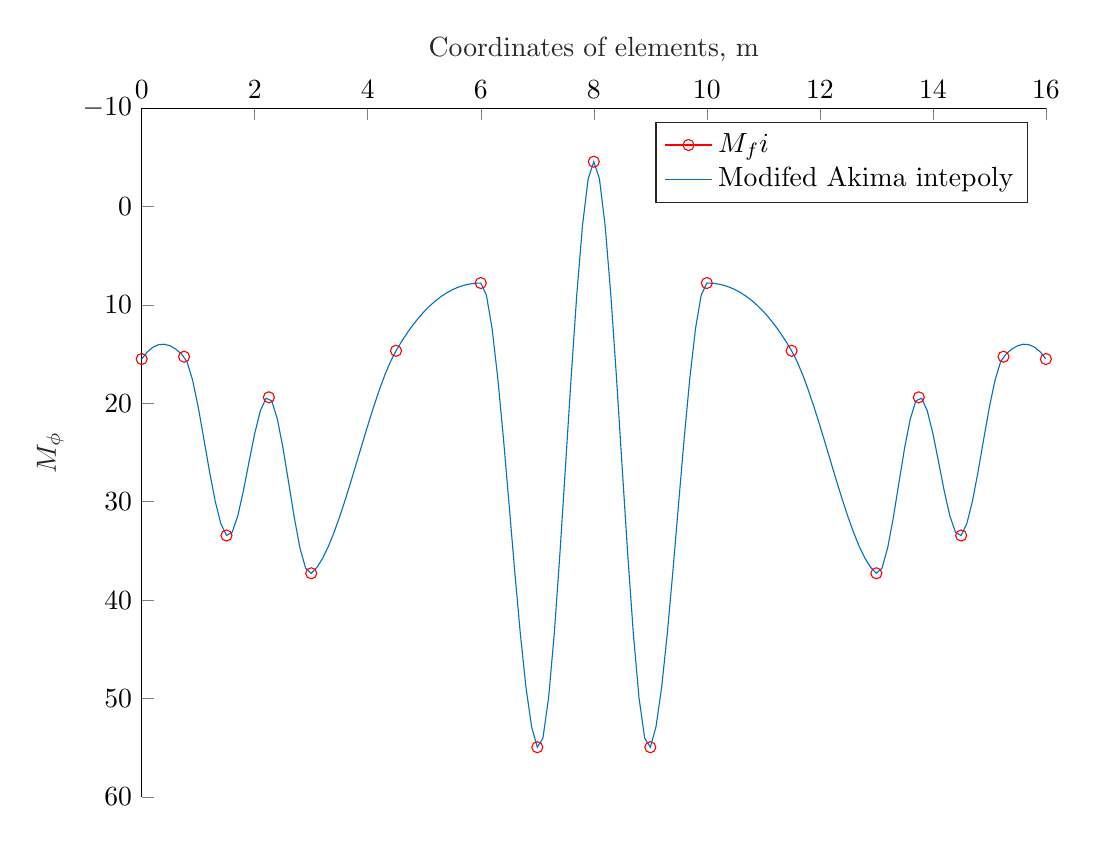
\begin{tikzpicture}

\begin{axis}[%
width=4.521in,
height=3.444in,
at={(0.758in,0.481in)},
scale only axis,
xmin=0,
xmax=16,
xlabel style={font=\color{white!15!black}},
xlabel={Coordinates of elements, m},
y dir=reverse,
ymin=-10,
ymax=60,
ylabel style={font=\color{white!15!black}},
ylabel={$\text{M}_{\phi}$},
axis background/.style={fill=white},
axis x line*=top,
axis y line*=left,
legend style={legend cell align=left, align=left, draw=white!15!black}
]
\addplot [color=red, draw=none, mark=o, mark options={solid, red}]
  table[row sep=crcr]{%
0	15.4994216772269\\
0.75	15.2634807239999\\
1.5	33.4321891857775\\
2.25	19.3935731642471\\
3	37.2763571271773\\
4.5	14.6628998937865\\
6	7.77659546991003\\
7	54.9516495541952\\
8	-4.55611328895156\\
9	54.9516495541952\\
10	7.77659546991003\\
11.5	14.6628998937865\\
13	37.2763571271773\\
13.75	19.3935731642471\\
14.5	33.4321891857775\\
15.25	15.2634807239999\\
16	15.4994216772269\\
};
\addlegendentry{$\text{M}_\text{f}\text{i}$}

\addplot [color=mycolor1]
  table[row sep=crcr]{%
0	15.4994216772269\\
0.1	14.7743740830793\\
0.2	14.2937664209717\\
0.3	14.0406743308349\\
0.4	13.9981734525996\\
0.5	14.1493394261965\\
0.6	14.4772478915563\\
0.7	14.9649744886097\\
0.8	15.7537774431237\\
0.9	17.6344095704744\\
1	20.3867266730786\\
1.1	23.6166888186756\\
1.2	26.9302560750047\\
1.3	29.9333885098051\\
1.4	32.2320461908163\\
1.5	33.4321891857775\\
1.6	33.1128112479404\\
1.7	31.4356422999828\\
1.8	28.8807466637829\\
1.9	25.928188661219\\
2	23.0580326141695\\
2.1	20.7503428445125\\
2.2	19.4851836741265\\
2.3	19.7380775236131\\
2.4	21.5835261895003\\
2.5	24.5302570138488\\
2.6	28.0495046713632\\
2.7	31.6125038367485\\
2.8	34.6904891847093\\
2.9	36.7546953899507\\
3	37.2763571271773\\
3.1	36.6791514960672\\
3.2	35.76761633084\\
3.3	34.5842774080135\\
3.4	33.1716605041054\\
3.5	31.5722913956333\\
3.6	29.828695859115\\
3.7	27.9833996710681\\
3.8	26.0789286080104\\
3.9	24.1578084464594\\
4	22.2625649629329\\
4.1	20.4357239339485\\
4.2	18.719811136024\\
4.3	17.1573523456771\\
4.4	15.7908733394253\\
4.5	14.6628998937865\\
4.6	13.7086249868383\\
4.7	12.8335844304415\\
4.8	12.0358182517883\\
4.9	11.3133664780709\\
5	10.6642691364814\\
5.1	10.0865662542121\\
5.2	9.57829785845523\\
5.3	9.13750397640293\\
5.4	8.76222463524741\\
5.5	8.45049986218088\\
5.6	8.20036968439553\\
5.7	8.00987412908358\\
5.8	7.87705322343721\\
5.9	7.79994699464863\\
6	7.77659546991003\\
6.1	9.01762643905283\\
6.2	12.394220929076\\
6.3	17.3952488229233\\
6.4	23.5095800035383\\
6.5	30.2260843538646\\
6.6	37.0336317568461\\
6.7	43.4210920954262\\
6.8	48.8773352525486\\
6.9	52.8912311111571\\
7	54.9516495541952\\
7.1	54.0252076485368\\
7.2	49.9318700963544\\
7.3	43.4405282335397\\
7.4	35.3200733959848\\
7.5	26.3393969195812\\
7.6	17.2673901402209\\
7.7	8.87294439379566\\
7.8	1.92495101619726\\
7.9	-2.80769865668239\\
8	-4.55611328895156\\
8.1	-2.80769865668239\\
8.2	1.92495101619727\\
8.3	8.87294439379574\\
8.4	17.2673901402208\\
8.5	26.3393969195812\\
8.6	35.3200733959848\\
8.7	43.4405282335397\\
8.8	49.9318700963544\\
8.9	54.0252076485368\\
9	54.9516495541952\\
9.1	52.8912311111571\\
9.2	48.8773352525486\\
9.3	43.4210920954261\\
9.4	37.0336317568461\\
9.5	30.2260843538646\\
9.6	23.5095800035383\\
9.7	17.3952488229233\\
9.8	12.394220929076\\
9.9	9.01762643905286\\
10	7.77659546991003\\
10.1	7.79994699464863\\
10.2	7.87705322343721\\
10.3	8.00987412908358\\
10.4	8.20036968439553\\
10.5	8.45049986218088\\
10.6	8.76222463524741\\
10.7	9.13750397640293\\
10.8	9.57829785845524\\
10.9	10.0865662542121\\
11	10.6642691364814\\
11.1	11.3133664780709\\
11.2	12.0358182517883\\
11.3	12.8335844304415\\
11.4	13.7086249868383\\
11.5	14.6628998937865\\
11.6	15.7908733394253\\
11.7	17.1573523456771\\
11.8	18.719811136024\\
11.9	20.4357239339485\\
12	22.2625649629329\\
12.1	24.1578084464594\\
12.2	26.0789286080103\\
12.3	27.9833996710682\\
12.4	29.828695859115\\
12.5	31.5722913956333\\
12.6	33.1716605041054\\
12.7	34.5842774080135\\
12.8	35.76761633084\\
12.9	36.6791514960672\\
13	37.2763571271773\\
13.1	36.7546953899507\\
13.2	34.6904891847094\\
13.3	31.6125038367484\\
13.4	28.0495046713632\\
13.5	24.5302570138488\\
13.6	21.5835261895003\\
13.7	19.7380775236131\\
13.8	19.4851836741265\\
13.9	20.7503428445126\\
14	23.0580326141695\\
14.1	25.928188661219\\
14.2	28.8807466637829\\
14.3	31.4356422999828\\
14.4	33.1128112479404\\
14.5	33.4321891857775\\
14.6	32.2320461908163\\
14.7	29.9333885098052\\
14.8	26.9302560750046\\
14.9	23.6166888186756\\
15	20.3867266730786\\
15.1	17.6344095704744\\
15.2	15.7537774431237\\
15.3	14.9649744886097\\
15.4	14.4772478915563\\
15.5	14.1493394261965\\
15.6	13.9981734525996\\
15.7	14.0406743308349\\
15.8	14.2937664209717\\
15.9	14.7743740830793\\
16	15.4994216772269\\
};
\addlegendentry{Modifed Akima intepoly}

\end{axis}
\end{tikzpicture}%
    \caption{ $M_{\varphi}$ across plate }
    \label{fig:UglobFull}
\end{figure}